%%%
%% Problem Analysis :: Problem
%%%
\section{Problem}

A typical crossword involves a grid with black squares, not to be filled in by
the  solver, and white squares used by the solver to input their answers. The
input comes from the solver working out the answer to given clues. These clues
have an orientation, a length and a number associated with its related position
within the grid. The fundamental difference between a typical crossword and a
cryptic crossword are the clues themselves.

Cryptic crosswords are a popular type of puzzles found in many parts of the
world. Most common-wealth national newspapers will print cryptic crosswords of
varying difficulty on a daily basis.

Cryptic crosswords are a unique style of crosswords, in which the answer to
each given clue is a word puzzle. An answer can only be obtained if the cryptic
clue is read in the correct way. Often when the clue is surface read, the clue
makes no sense at all. The challenge is to find a way in which the reading of
the clue leads to a solution. To aid with solving cryptic crosswords, the clues
are written to be within specific categories, such as reversals and anagrams,
which have individual characteristics.

Many users can often become frustrated when a clue appears to be unsolvable. It
is the vast range of possible clues that often makes solving not only
challenging but interesting as well.

Fundamentally, the overall aim of this project is to develop a piece of
software that is able to solve any given type of cryptic crossword clue.


%%%
%% Problem Analysis :: Product
%%%
\section{Product}

Within this group project, three components will be delivered. The first 
deliverable is the final, working piece of software. Whilst the second and third
deliverables are written reports. The second deliverable is a group written 
report comprising of the all research and implementation details of the software
product. The final deliverable will be each member's individual analysis and 
evolution of the project as a whole.

Based upon the given background and problem information it could be possible to
develop a product that is able to solve the given problem.

The final product would be a piece of software that is able to understand a
given clue and try to deduce what the answer to the clue is. This would require
the software to have some form of natural language processing component as well
as one or more cryptic crossword algorithms. Once a clue has been correctly
``guessed'' it can simply be returned to the user. It is the ``guessing'' of
the answer that this project will primarily focus upon.

In order to gain maximum user coverage, the software must have an easy to use
interface. The main reason for this is that the computer literacy of the
intended users is not known - although basic computer literacy is assumed.


%%%
%% Problem Analysis :: Client and Stakeholders
%%%
\section{Client \& Stakeholders}

Dr Hugh Osborne, a lecturer from the University of Huddersfield will be the
client for the group project. Dr Hugh Osborne has a keen interest in cryptic
crosswords and the problem in the area which the group intends to help to
eliminate. The role of the client for the group project will be to input ideas
and potential requirements which Hugh, as an experienced solver of cryptic 
crosswords, would consider to be necessary. As a client for the project, Hugh 
will also be present for academic demonstrations.

Dr Gary Allen, Dr Sotirios Batsakis and Dr Colin Venters, all lecturers at the
University of Huddersfield, will act as stakeholders for the group project. Gary
will be the most involved external individual as the project supervisor. The 
role of project supervisor requires frequent meetings with the team to monitor 
the development of the project, provide guidance as well as opinion on certain 
aspects of the life cycle.

Sotirios and Colin will have a less active role within the project during the
project life cycle than the role of the client or the project supervisor.  These
stakeholders will play active roles at particular milestones of the group
project such as providing guidance for the proposal of the project and at the
project demonstration approximately half way through the life cycle.


%%%
%% Problem Analysis :: Users
%%%
\section{Users} 

Kathryn Friedlander and Philip Fine \citep{friedlander09} carried out an
investigation into whether the amount of cryptic crosswords completed by a
solver determined how successful they were at solving them. To complete this
study they gathered data from 241 people and have deduced the following facts 
about the user base \citep{friedlander09}:

\begin{itemize}
  \item ``209 M, 32 F''
  \item ``mean age=53 years, range=23 -- 83''
  \item ``mean time spent=8 hours per week, range=1-30''
\end{itemize}

To support decisions made within the project life cycle an additional
quantitative research method has been utilized to gain a larger understanding
of the types of users the deliverable will attract. The research method used by 
the team is in the form of a survey. 

The survey results gathered were seen as additional justifications for the 
purpose of the project. Moreover, data collected from the survey was expected to
indicate the locations in which users complete cryptic crosswords to understand 
the potential need for the deliverable to be of a transportable nature.

The following questions were asked:

\begin{enumerate}
  \item Do you play Cryptic Crosswords?
  \item How often do you play?
  \item How do you complete cryptic crosswords? % Where do you play?
  \item Do you often finish them?
  \item If no to the previous question, what reason don't you finish them?
  \item What is your age group?
  \item When do you play Cryptic Crosswords?
  \item What gender are you?
  \item What is the Highest qualification you have?
  \item What platform is your mobile phone on?
\end{enumerate}

The survey was conducted between 18th November and 4th January. It was 
distributed across the University of Huddersfield portal message board,
Facebook and Twitter.


%%%
%% Problem Analysis :: Users :: Results
%%%
\subsection{Results}

The survey that was outlined within the previous section managed to provide some
interesting trends. Within this subsection a number of the trends will be 
highlighted, and discussed. It is hoped that the trends will be able to help 
guide the research, design and development processes throughout the project.

One of the key questions that was asked within the survey was ``how do you 
complete cryptic crosswords?'', which the question referred to the format in 
which users generally tended to play or favour. 

Figure \ref{fig:playing_format} illustrates the responses from the question. The
over all statement is that 56\% of those surveyed favoured a paper based format
which perhaps is a little surprising in today's `digital age'.

\begin{figure}[H]
  \centering
  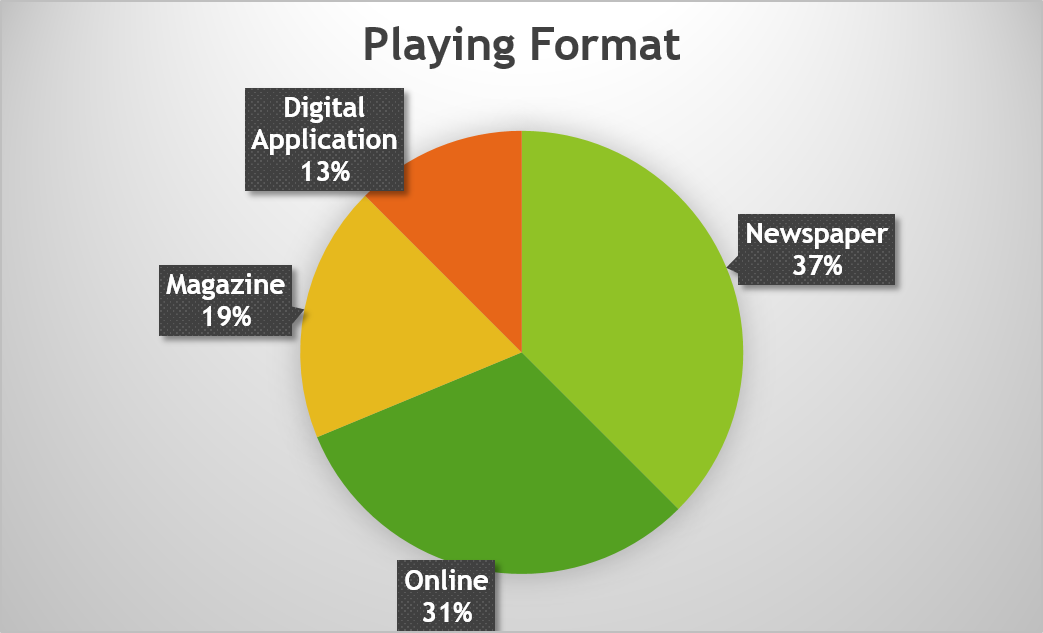
\includegraphics[scale=0.9]{graphs/playing_format.png}
  \caption{Pie chart illustrating how users complete cryptic crosswords}
  \label{fig:playing_format}
\end{figure}

Following on from this it was also surprising that very few individuals use a 
mobile-based application to complete cryptic crosswords --- especially as 
on-line crosswords were the second most used format. It is this area that is
intended to be a large basis for this project, and hence this will need to be
investigated thoroughly.

The survey also tried to deduce the reasons behind why cryptic crossword users 
are perhaps sometimes unable to solve a clue. The understanding of the responses
to this question is a critical part of the project, as that it is intended that
the final product should be able to solve a given clue, and thus help a solver.

Figure \ref{fig:incomplete} illustrates the responses from all users --- both 
advanced and basic users. The chart shows that the most common reason as to why
users are unable to complete crosswords is that they don't have the time to 
complete the crossword --- something that the project may not be able to 
directly solve.

\begin{figure}[H]
  \centering
  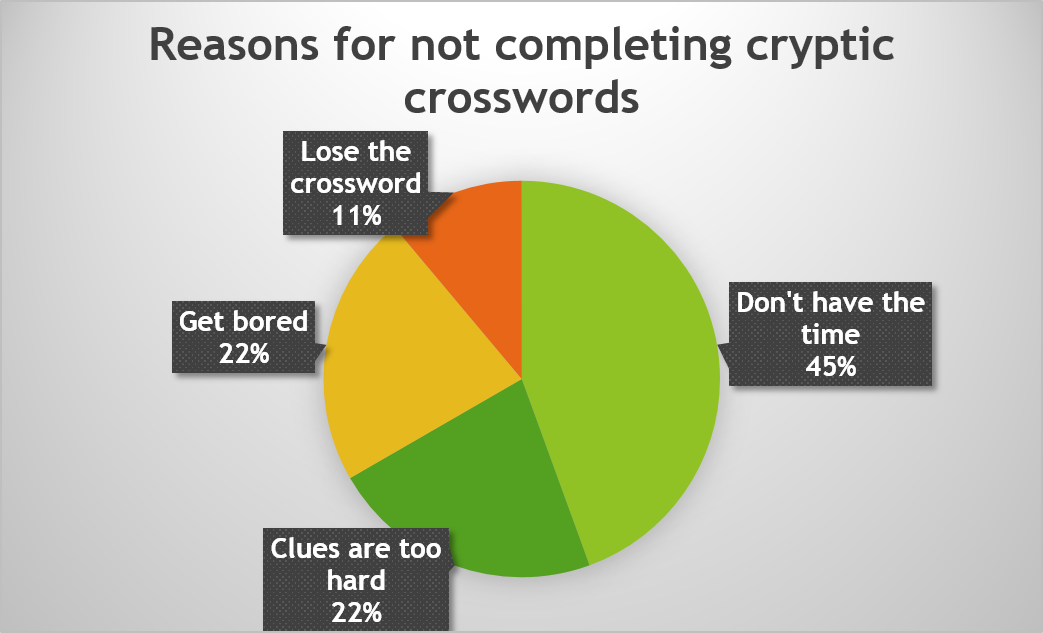
\includegraphics[scale=0.9]{graphs/incomplete.png}
  \caption{Pie chart illustrating why all users are unable to complete cryptic 
          crosswords}
  \label{fig:incomplete}
\end{figure}

However the next top two responses --- ``clues are too hard'' and ``get bored'' 
--- could be attempted to be solved within this project. These two responses 
could be linked together, for example do users get bored because the clues are 
too hard? Although the survey did not highlight this, it did illustrate a 
potential trend in the data that can be invested further.

Figure \ref{fig:incomplete} illustrated responses from all users, if 
``advanced users'' are removed then a more clear trend may emerge. For the 
purposes of this test an ``advanced user'' can be defined as a user who 
regularly tries to solve a cryptic crossword.

Figure \ref{fig:incompleted} illustrates responses only from ``basic users''. 
Although the overall trend is the same, it does highlight a larger gap between 
the two other responses --- ``clues are too hard'' and ``get bored''. 

\begin{figure}[H]
  \centering
  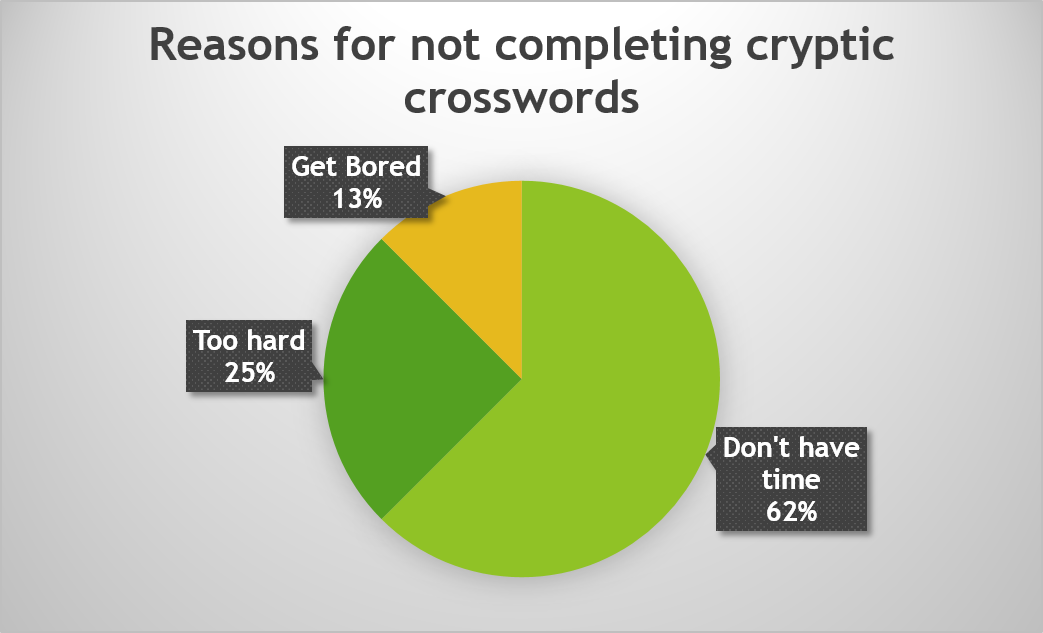
\includegraphics[scale=0.9]{graphs/incomplete_2.png}
  \caption{Pie chart illustrating why basic users are unable to complete cryptic
          crosswords}
  \label{fig:incompleted}
\end{figure}

This identifies another possible trend in that users who can't solve clues may 
wish to `learn' how to solve that clue. This factor will need to be taken in to
consideration through the remainder of the project.

Additionally the survey tried to deduce when cryptic crosswords are completed. 
Figure \ref{fig:when_solved} illustrates the responses. Generally speaking it 
could be said that cryptic crosswords are completed to ``pass time''. The top 
two answers indicated that users completed crosswords when ``bored'' or 
``travelling''.

\begin{figure}[H]
  \centering
  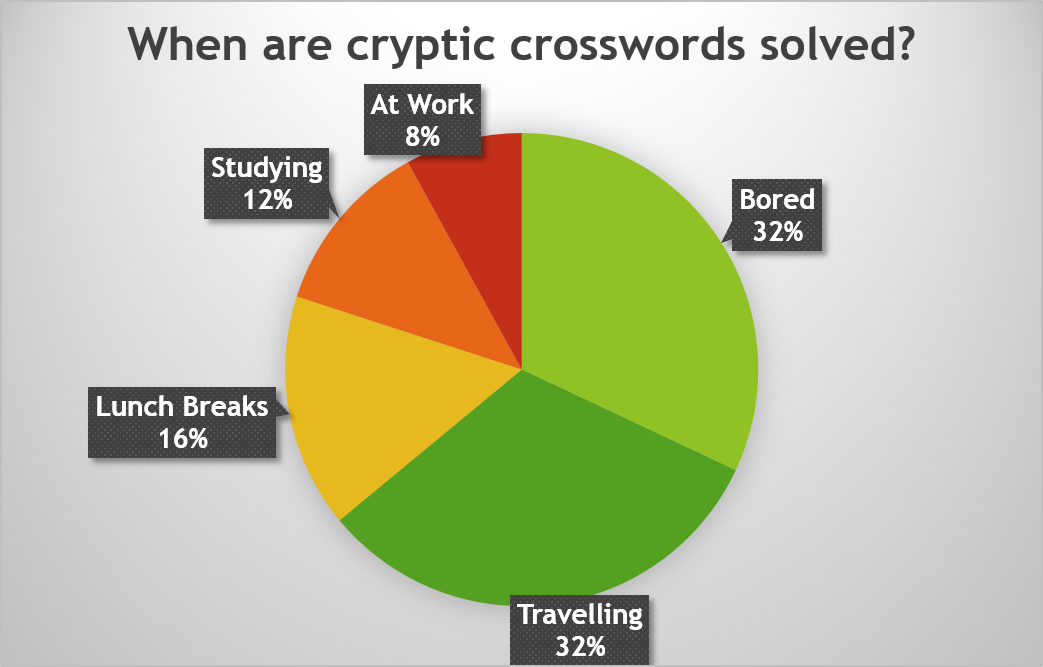
\includegraphics[scale=0.9]{graphs/when_solved.png}
  \caption{Pie chart illustrating when cryptic crosswords are solved}
  \label{fig:when_solved}
\end{figure}

The responses to the question were quite important, as it highlights that the 
responses are people who could be categorised as people who are ``on the go''. 
This means that they are not fixed in one location, such as travelling from home
to work back home again. Furthermore it highlights that there may be a potential
gap in the market for a mobile based application to aid in the solving of 
cryptic crosswords.

With this in mind, the final question tried to deduce which mobile platforms 
users owned and used. Figure \ref{fig:survey_os} illustrates the responses, and 
unsurprisingly the top two platform choices was Apple's iOS and Google's Android
operating systems.

\begin{figure}[H]
  \centering
  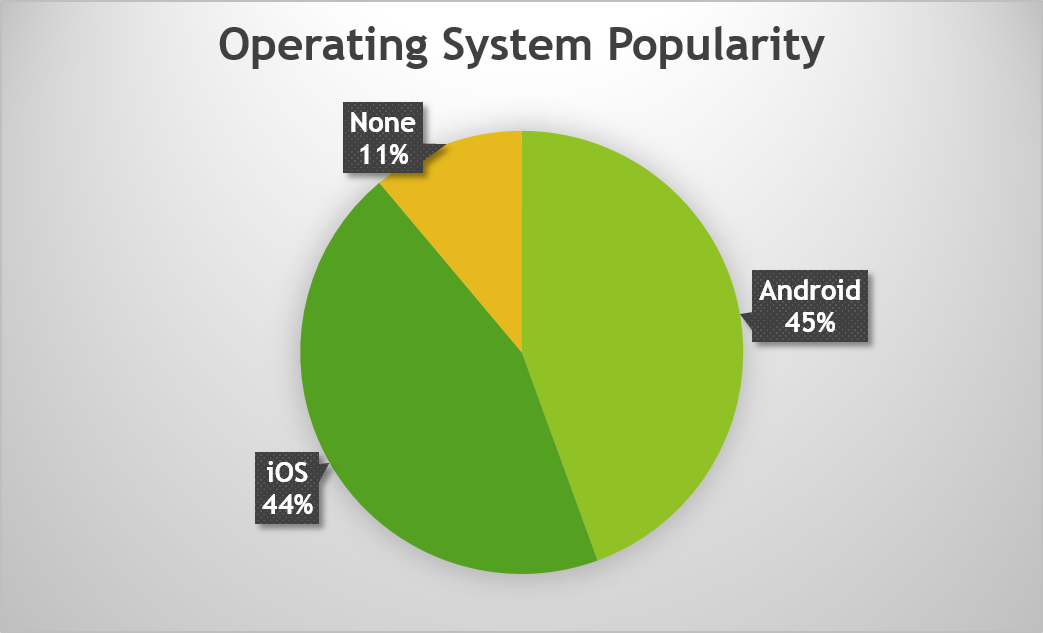
\includegraphics[scale=0.9]{graphs/operating_system.png}
  \caption{Pie chart illustrating the ownership of mobile devices by operating 
          system}
  \label{fig:survey_os}
\end{figure}

The chart indicates that if a mobile-based application was feasible then the 
application should run on at least iOS or Android.

~\\

The responses and results presented from the survey will be used to direct the 
`formal' academic research that will form part of the written deliverable of the
project. The specific research areas will be covered in the following section.
